\usepackage{graphicx}
\title{Introduction}
\begin{document}

\section{Analog vs. Digital}

\subsection {Infinite Information}

\begin{frame}{Infinite information}
  \begin{center}
    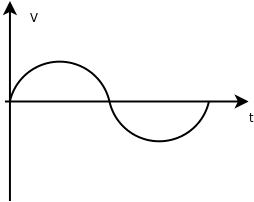
\includegraphics[height=5cm]{AnalogCurve.png}
  \end{center}
\end{frame}

\begin{itemize}
  \item We have a lot of information here, in fact, an infinite amount of information.
  \item Although this information is very useful, it may be more than we need for some applications.
\end{itemize}

\subsection{Key Engineering Concept}

\begin{frame}{Key engineering concept: simplify}
  \begin{block}{Engineering Concept}
    When faced with a complex problem, attempt to break the problem down into its simplest parts.
  \end{block}
  \begin{block}{Question}
    What is the minimum useful information we can use from the time varying voltage curve?
  \end{block}
\end{frame}

\begin{frame}{Logic values}
  \begin{center}
    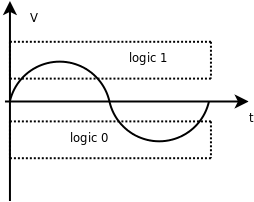
\includegraphics[height=5cm]{AnalogCurveWithLogicLevels.png}
  \end{center}
\end{frame}

\begin{itemize}
  \item Now we have a much more manageable situation, the signal is either on or off, 1 or 0.
  \item Notice that 1 and 0 are not fixed voltage values, but instead can be a range of values.
\end{itemize}

\begin{frame}{A digital signal}
  \begin{center}
    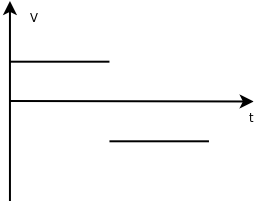
\includegraphics[height=5cm]{DigitalCurve.png}
  \end{center}
\end{frame}

\begin{itemize}
  \item We will not discuss analog signals much more in this course.  We will assume that they are digital.
  \item We must be aware that really, the signals are analog, and the operation of the digital circuits we will explore is subject to specified operating conditions, such as temperature and input voltage.
\end{itemize}

\section{Integrated Circuits}

\subsection{Integrated Circuit Types}

\begin{frame}{Gates}
  \begin{definition}
    A \alert{combinational circuit} is an digital circuit which produces an output based only the current combination of its input values.
  \end{definition}
  \begin{block}{Fundamental Gates}
    These gates are simple combinational circuits that serve as the building blocks for all digital circuits.
  \end{block}
  \begin{columns}
    \begin{column}{3cm}
      \begin{center}
        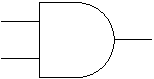
\includegraphics{ANDGate}
        \\AND gate
      \end{center}
    \end{column}
    \begin{column}{3cm}
      \begin{center}
        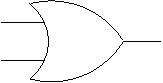
\includegraphics{ORGate}
        \\OR gate
      \end{center}
    \end{column}
    \begin{column}{3cm}
      \begin{center}
        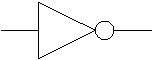
\includegraphics{NOTGate}
        \\NOT gate (inverter)
      \end{center}
    \end{column}
  \end{columns}
\end{frame}

\begin{frame}{How do these gates work?}
  \begin{block}{Truth table}
    The behavior of each gate is described by a \alert{truth table}.  The truth table lists all of the possible input combinations to the gate and the output for each input combination.
  \end{block}
  \vspace{5mm}
  \begin{columns}
    \begin{column}{3cm}
      \begin{center}
        AND gate\\
        \begin{tabular}{cc|c}
          \textbf{A} & \textbf{B} & \textbf{C} \\
          \hline
          0 & 0 & 0 \\
          0 & 1 & 0 \\
          1 & 0 & 0 \\
          1 & 1 & 1 \\
        \end{tabular}
      \end{center}
    \end{column}
    \begin{column}{3cm}
      \begin{center}
        OR gate\\
        \begin{tabular}{cc|c}
          \textbf{A} & \textbf{B} & \textbf{C} \\
          \hline
          0 & 0 & 0 \\
          0 & 1 & 1 \\
          1 & 0 & 1 \\
          1 & 1 & 1 \\
        \end{tabular}
      \end{center}
    \end{column}
    \begin{column}{3cm}
      \begin{center}
        NOT gate\\
        \begin{tabular}{c|c}
          \textbf{A} & \textbf{B} \\
          \hline
          0 & 1 \\
          1 & 0 \\
        \end{tabular}
      \end{center}
    \end{column}
  \end{columns}
\end{frame}

\begin{itemize}
  \item These three simple gates will be combined in many ways to build complex digital circuits.
  \item Note the application of our engineering principle again, make things simple first in order to solve complex problems.
  \item Note also that this is not simplification for the sake of simplification, but simplification to fundamental, basic principles, AND, OR, and NOT.  These concepts are the basic building blocks of relationships.
  \item For instance, these gates can be combined to create an entirely new type of circuit, called a sequential circuit.
\end{itemize}

\begin{frame}{Memory}
  \begin{definition}
    A \alert{sequential circuit} is a circuit which defines its output in terms of its current and past inputs, i.e. it has memory.
  \end{definition}
  \begin{block}{Flip-flop}
    A \alert{flip-flop} is a type of sequential circuit that stores either a 0 or a 1.  The value a flip-flop currently stores is called its \alert{state}.
  \end{block}
\end{frame}

\begin{frame}{Integrated Circuits}
  \begin{definition}
    An \alert{integrated circuit} is a collection of one or more gates on a silicon chip.
  \end{definition}
  \begin{itemize}
    \item SSI ICs are small-scale integration ICs - they contain up to 20 gates
    \item MSI ICs are medium-scale integration ICs - they contain up to 200 gates
    \item LSI ICs are large-scale integration ICs - they contain up to 1,000,000 gates
    \item VLSI ICs are very large-scale integration ICs - they contain millions of transistors 
  \end{itemize}
\end{frame}

\subsection{PLDs, ASICs, and PCBs}

\begin{frame}{PLDs and ASICs and PCBs, oh my!}
  \begin{block}{Programmable Logic Devices}
    Programmable logic devices (\alert{PLDs}) are arrays of gates which can be programmed and reprogrammed on the fly.
  \end{block}
  \begin{block}{Application-specific Integrated Circuits}
    Application-specific integrated circuits (\alert{ASICs}) are integrated circuits designed for a particular product or application.
  \end{block}
  \begin{block}{Printed Circuit Boards}
    Printed circuit boards (\alert{PCBs}) are laminated fiberglass boards that connect multiple ICs together using very thin traces.
  \end{block}
\end{frame}

\subsection{Hardware Description Language}

\begin{frame}{Using software to create hardware}
  \begin{block}{Hardware Description Language}
    A hardware description language (\alert{HDL}) is a programming language that is used to design and test hardware.  HDLs are usually paired with PLDs to allow hardware to be quickly designed and tested.
  \end{block}
  \begin{itemize}
    \item VHDL
    \item Verilog
    \item Abel
  \end{itemize}
\end{frame}

\end{document}
